% latex table generated in R 3.6.3 by xtable 1.8-4 package
% Thu Jan 18 11:46:31 2024
\begin{table}[ht]
\centering
\begin{tabular}{rlrrr}
  \hline
 & OTU & MeanRA & MedianRA & SE \\ 
  \hline
1479019 & Methylobacterium sp. C & 0.00007145 & 0.00007394 & 0.00000476 \\ 
  440085 & Methylorubrum extorquens & 0.00006799 & 0.00006275 & 0.00000874 \\ 
  419610 & Methylorubrum extorquens & 0.00006332 & 0.00005219 & 0.00001119 \\ 
  207340 & Roseomonas mucos & 0.00006025 & 0.00005988 & 0.00000270 \\ 
  634177 & Komagataeibacter medellinensis & 0.00004547 & 0.00004773 & 0.00000312 \\ 
  2592655 & Acetobacter vaccini & 0.00003791 & 0.00003992 & 0.00000195 \\ 
  215743 & Roseovarius mucosu & 0.00002171 & 0.00002091 & 0.00000138 \\ 
  681157 & Phaeobacter sp. LSS & 0.00001184 & 0.00001180 & 0.00000099 \\ 
  655307 & Neisseria sp. KEM23 & 0.00004265 & 0.00004194 & 0.00000225 \\ 
  2749999 & Pseudomonas sp. RtIB02 & 0.00004923 & 0.00004536 & 0.00000386 \\ 
  1173270 & Pseudomonas sp. R1-43-0 & 0.00000455 & 0.00000310 & 0.00000110 \\ 
  29442 & Pseudomonas tolaasi & 0.00004057 & 0.00003643 & 0.00000427 \\ 
  384676 & Pseudomonas entomophila & 0.00007524 & 0.00007304 & 0.00000675 \\ 
  237609 & Pseudomonas alkylphenolic & 0.00008217 & 0.00007789 & 0.00000699 \\ 
  797277 & Halopseudomonas litorali & 0.00006449 & 0.00005964 & 0.00000393 \\ 
  1434072 & Halopseudomonas salegen & 0.00005118 & 0.00005081 & 0.00000382 \\ 
  163011 & Pseudomonas lin & 0.00003309 & 0.00003403 & 0.00000244 \\ 
  1812935 & Enterobacter roggenkampi & 0.00002745 & 0.00002598 & 0.00000200 \\ 
  1134687 & Klebsiella michiganensi & 0.00003654 & 0.00004384 & 0.00000613 \\ 
  55211 & Erwinia persicin & 0.00002654 & 0.00002583 & 0.00000127 \\ 
  1223571 & Dickeya chrysanthemi & 0.00000697 & 0.00000523 & 0.00000147 \\ 
  930806 & Halioglobus pacificu & 0.00005583 & 0.00005317 & 0.00000312 \\ 
  75293 & Streptomyces autolyticu & 0.00005368 & 0.00004622 & 0.00001002 \\ 
  1929477 & Streptomyces solisilva & 0.00004335 & 0.00004056 & 0.00000379 \\ 
  43675 & Rothia mucilaginos & 0.00005378 & 0.00005094 & 0.00000386 \\ 
  29311 & Mycobacterium haemophilu & 0.00007385 & 0.00007477 & 0.00000547 \\ 
  89154 & Corynebacterium terpenotabidu & 0.00007017 & 0.00007418 & 0.00000478 \\ 
  1404244 & Corynebacterium glyciniphilu & 0.00006575 & 0.00006151 & 0.00000448 \\ 
  169292 & Corynebacterium aurimucosu & 0.00004098 & 0.00003862 & 0.00000324 \\ 
  39791 & Corynebacterium glucuronolyticu & 0.00004552 & 0.00004623 & 0.00000332 \\ 
  203263 & Corynebacterium aquila & 0.00003262 & 0.00003059 & 0.00000319 \\ 
  161899 & Corynebacterium singular & 0.00002044 & 0.00002042 & 0.00000231 \\ 
  1408191 & Corynebacterium desert & 0.00001642 & 0.00001569 & 0.00000130 \\ 
  40567 & Actinosynnema miru & 0.00002692 & 0.00002806 & 0.00000173 \\ 
  1960083 & Actinomyces gaoshouyi & 0.00004758 & 0.00004792 & 0.00000302 \\ 
  2631020 & Arcanobacterium & 0.00002683 & 0.00002579 & 0.00000203 \\ 
  44251 & Paenibacillus duru & 0.00007401 & 0.00007245 & 0.00000652 \\ 
  1619311 & Paenibacillus physcomitrella & 0.00002961 & 0.00003136 & 0.00000242 \\ 
  189425 & Paenibacillus gramini & 0.00001730 & 0.00001709 & 0.00000124 \\ 
  714067 & Kroppenstedtia eburne & 0.00006965 & 0.00004316 & 0.00001707 \\ 
  33943 & Kyrpidia tuscia & 0.00002535 & 0.00002450 & 0.00000167 \\ 
  208479 & Enterocloster boltea & 0.00001634 & 0.00001709 & 0.00000202 \\ 
  1323375 & Anoxybacter fermentan & 0.00001798 & 0.00001841 & 0.00000184 \\ 
  224012 & Nostoc piscinal & 0.00001339 & 0.00000940 & 0.00000329 \\ 
  2518495 &   & 0.00003594 & 0.00003584 & 0.00000157 \\ 
  2715679 & Dissulfurispira thermophil & 0.00001363 & 0.00001358 & 0.00000199 \\ 
  515635 & Dictyoglomus turgidum & 0.00001716 & 0.00001769 & 0.00000184 \\ 
  2269 & Thermofilum penden & 0.00000625 & 0.00000771 & 0.00000093 \\ 
  69223 & Musicola paradisiac & 0.00003078 & 0.00003399 & 0.00000534 \\ 
   \hline
\end{tabular}
\caption{Keystone OTUs of } 
\end{table}
\begin{figure}
\centering
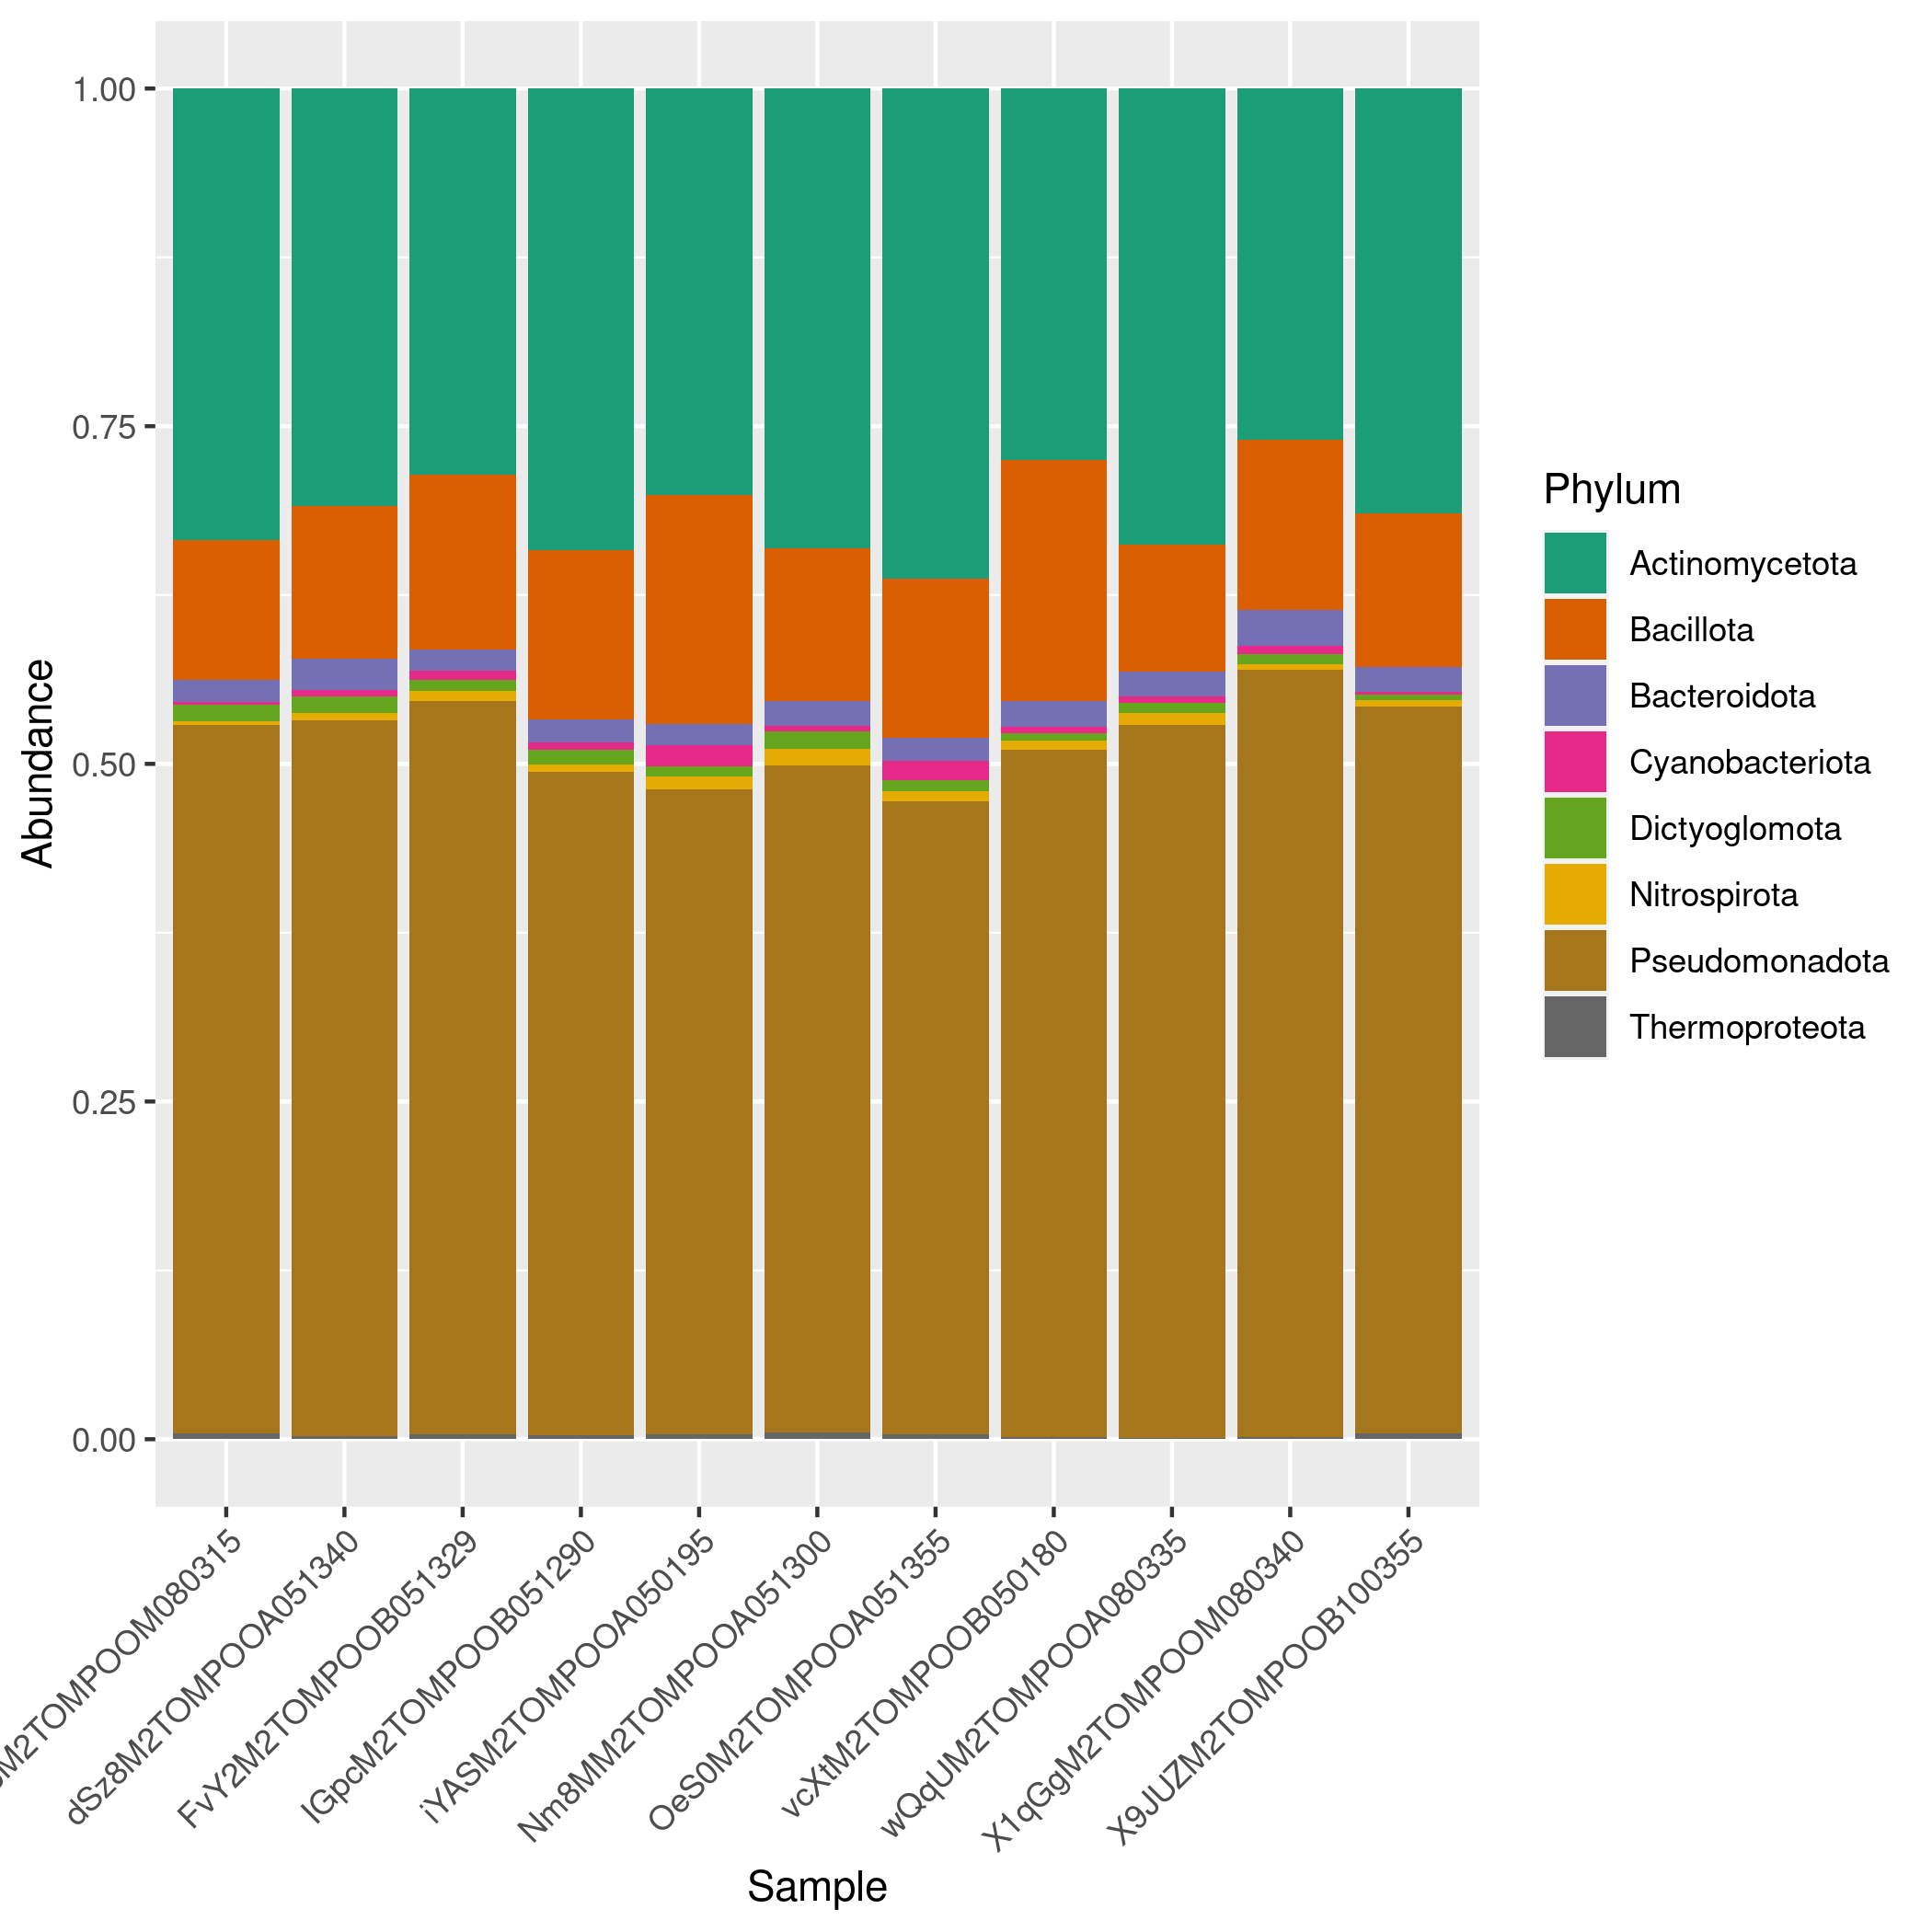
\includegraphics[scale = 0.8]{tomate_aleatorio1_2.csv_relative_abundance_Phylum.png}
\caption{Relative abundance by phyla of keystone OTUs }
\label{fig:tomate_aleatorio1_2.csv_phyla}
\end{figure}
\begin{figure}
\centering
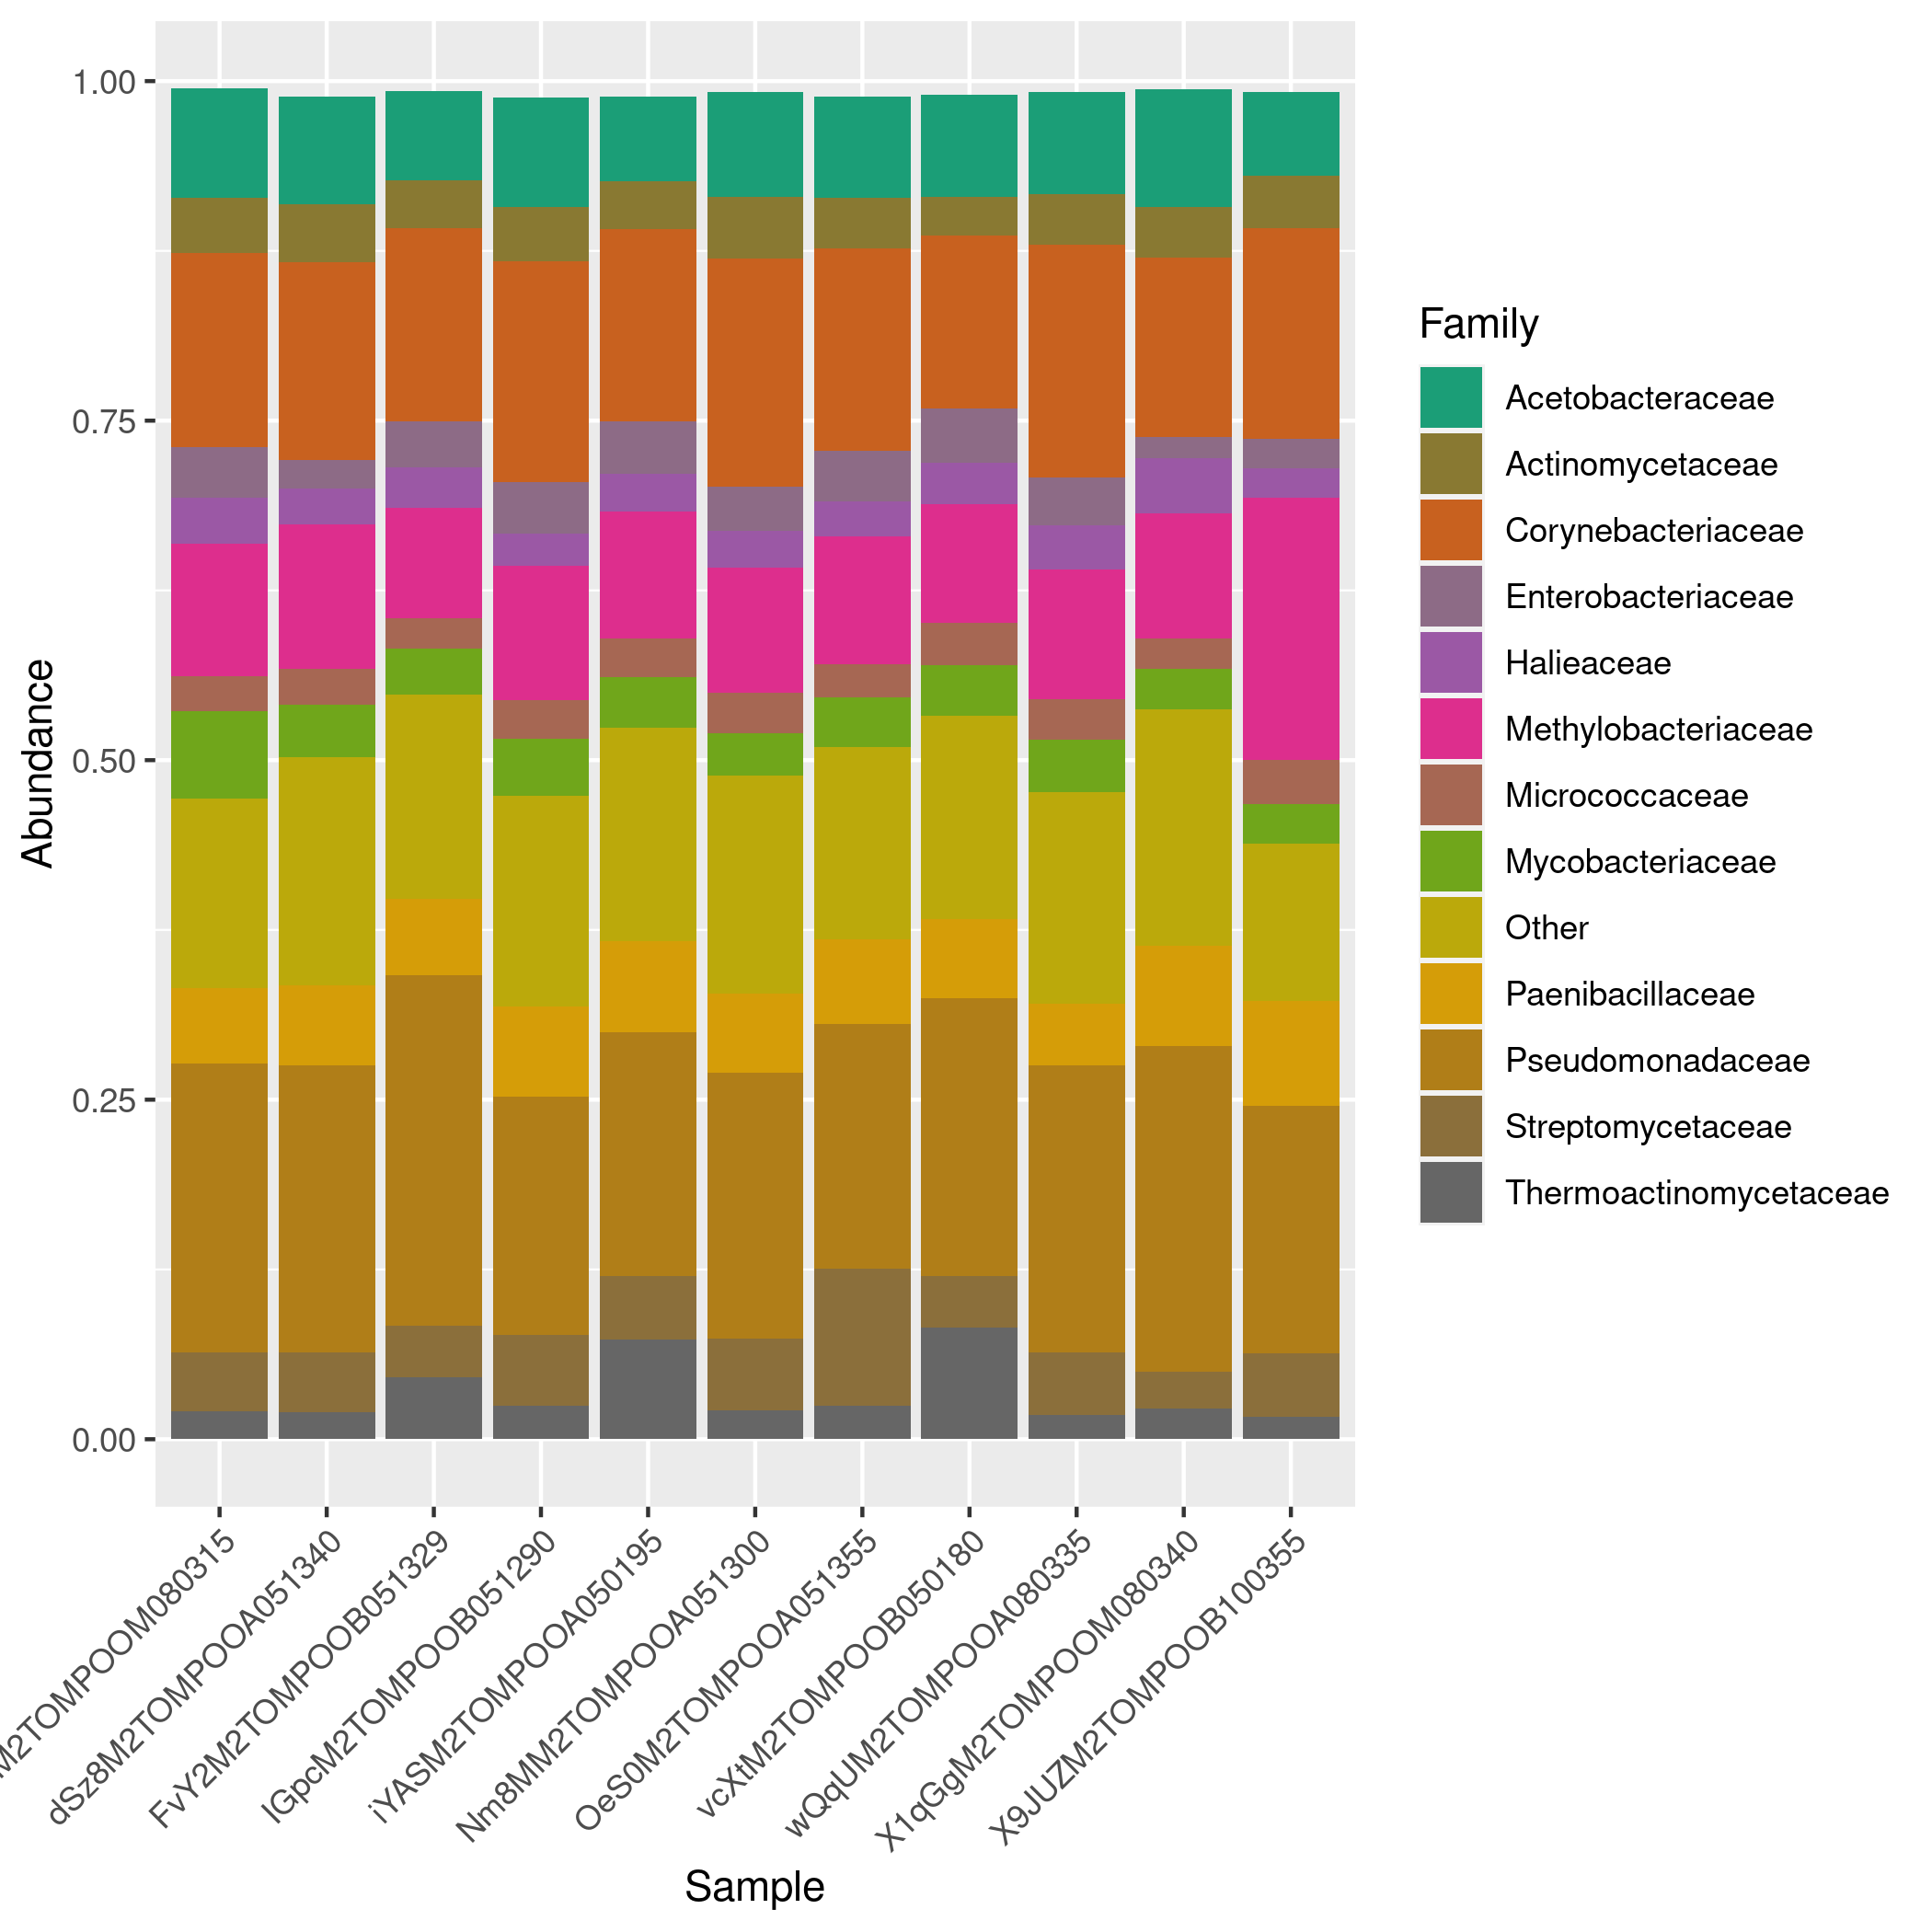
\includegraphics[scale = 0.8]{tomate_aleatorio1_2.csv_relative_abundance_Family.png}
\caption{Relative abundance by families of keystone OTUs }
\label{fig:tomate_aleatorio1_2.csv_family}
\end{figure}
\begin{figure}
\centering
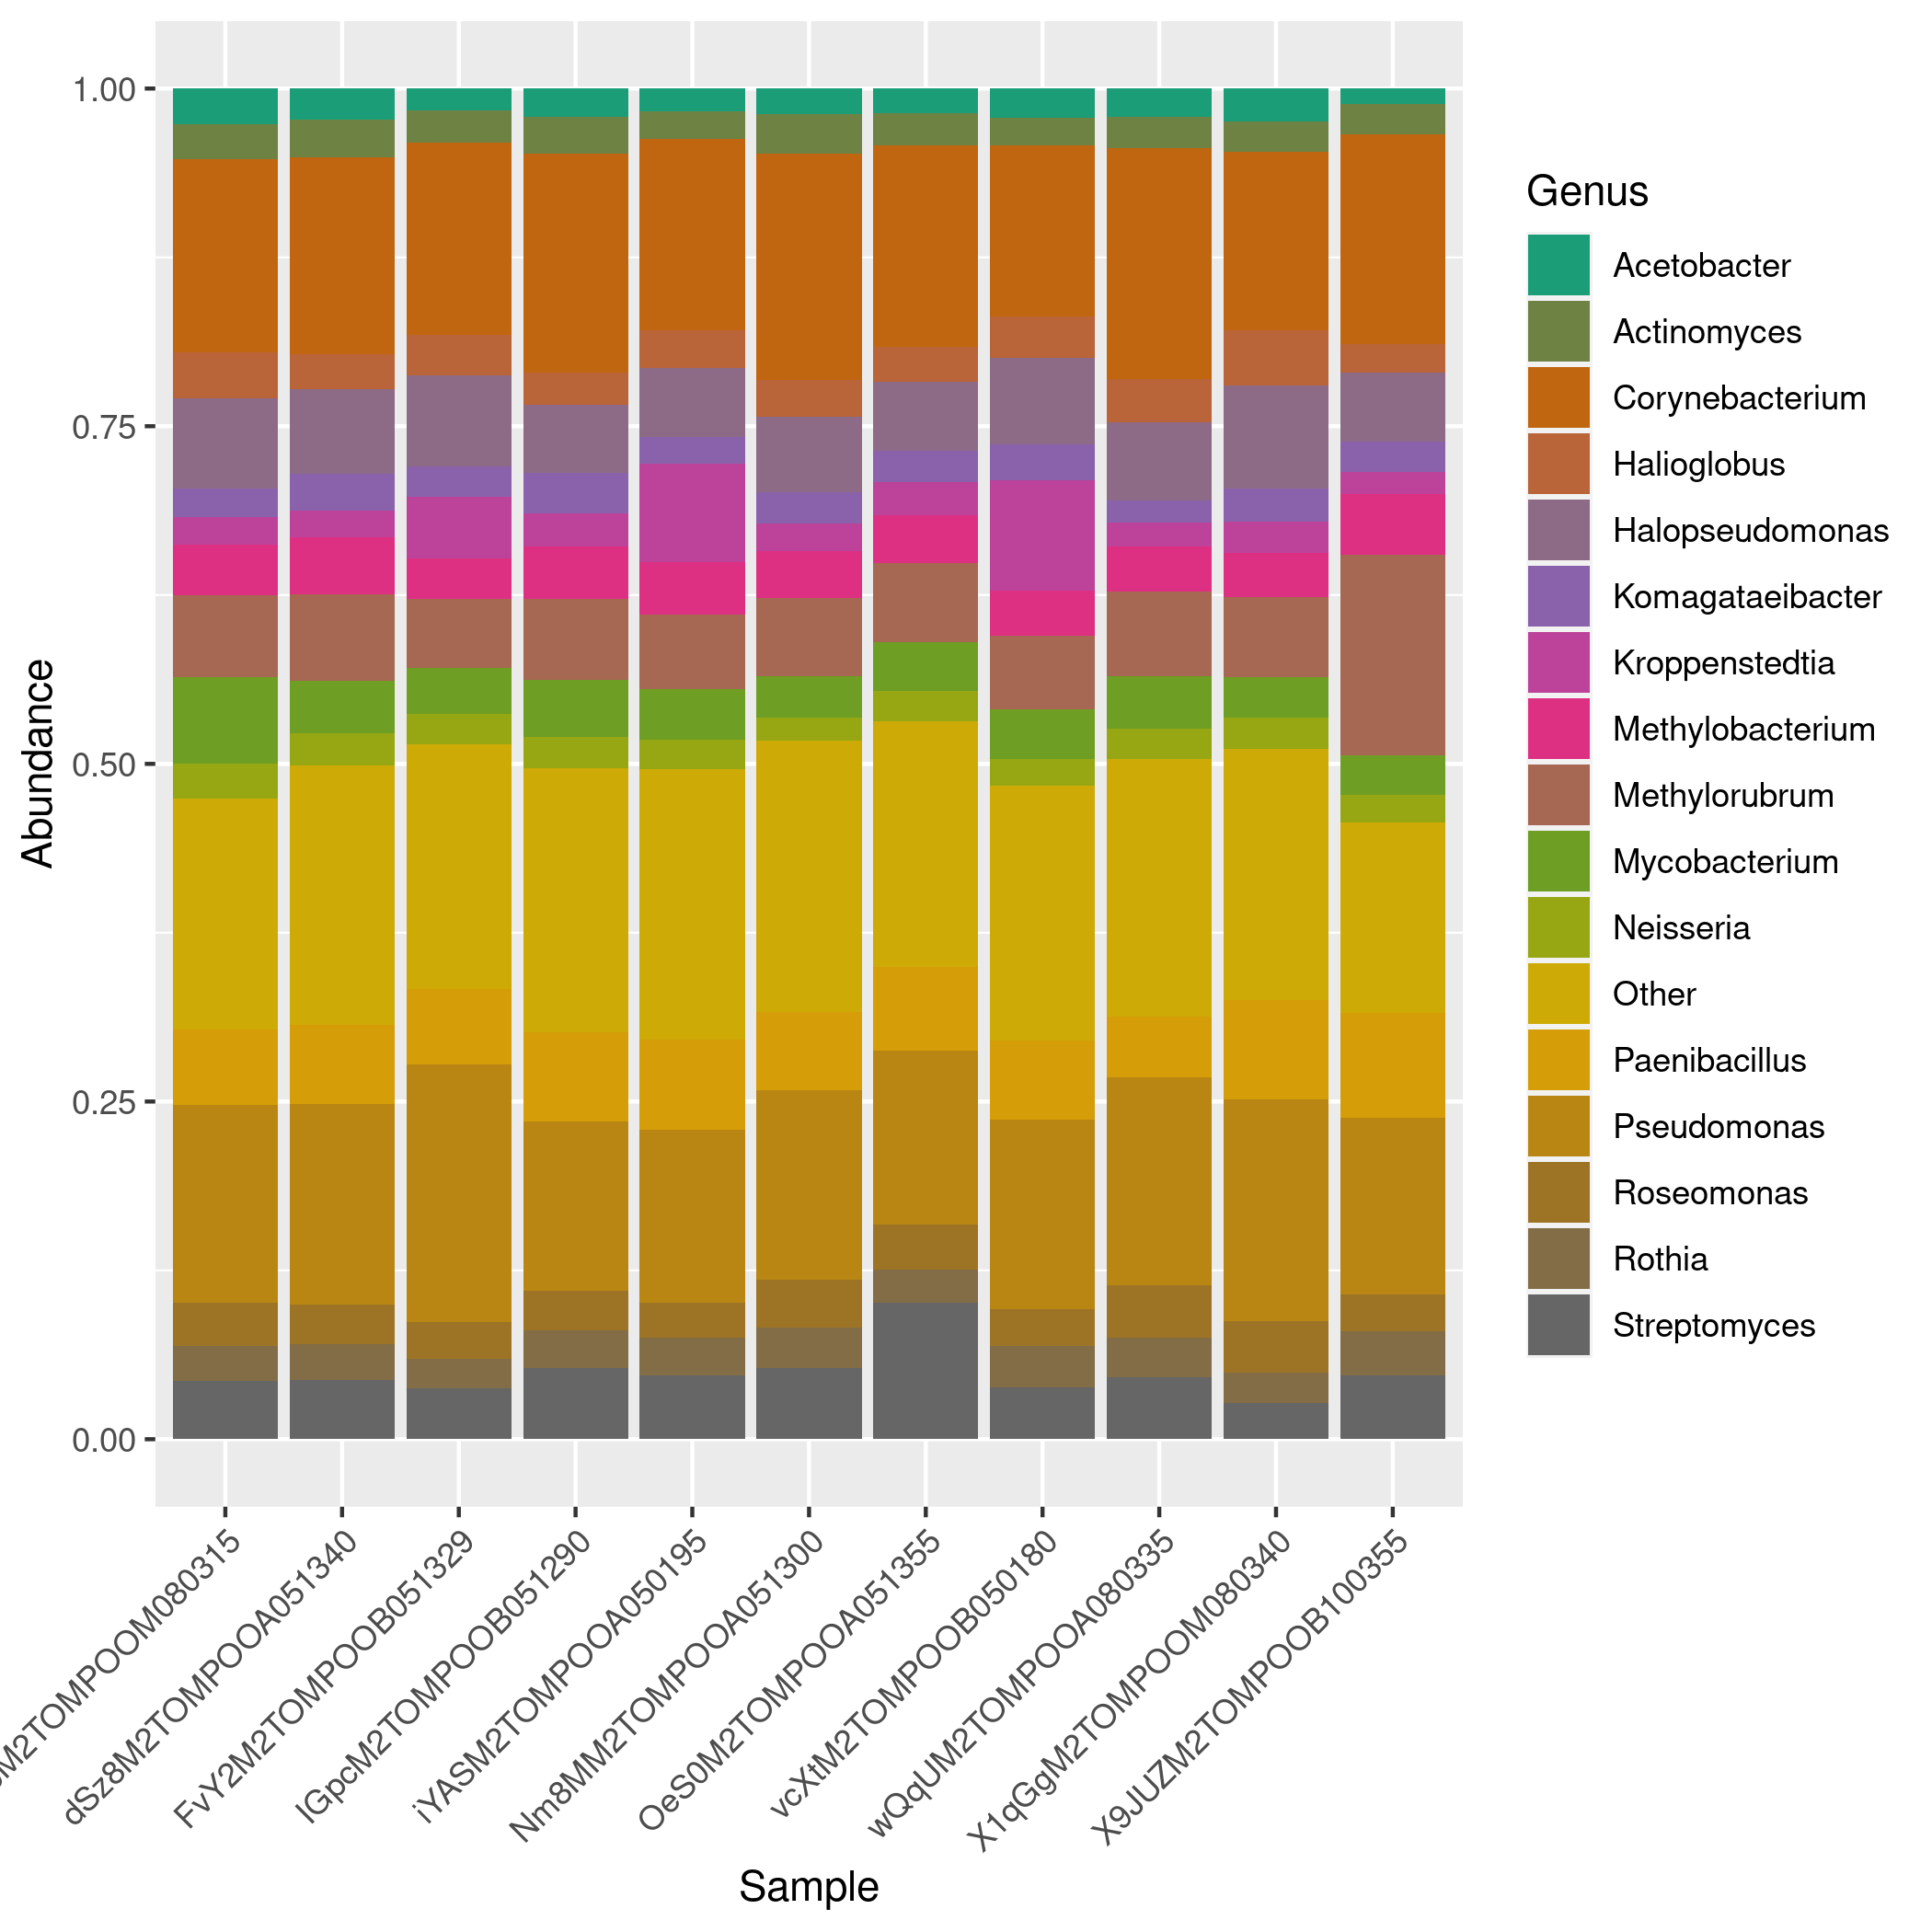
\includegraphics[scale = 0.8]{tomate_aleatorio1_2.csv_relative_abundance_Genus.png}
\caption{Relative abundance by genera of keystone OTUs }
\label{fig:tomate_aleatorio1_2.csv_genus}
\end{figure}
\begin{figure}
   \centering
   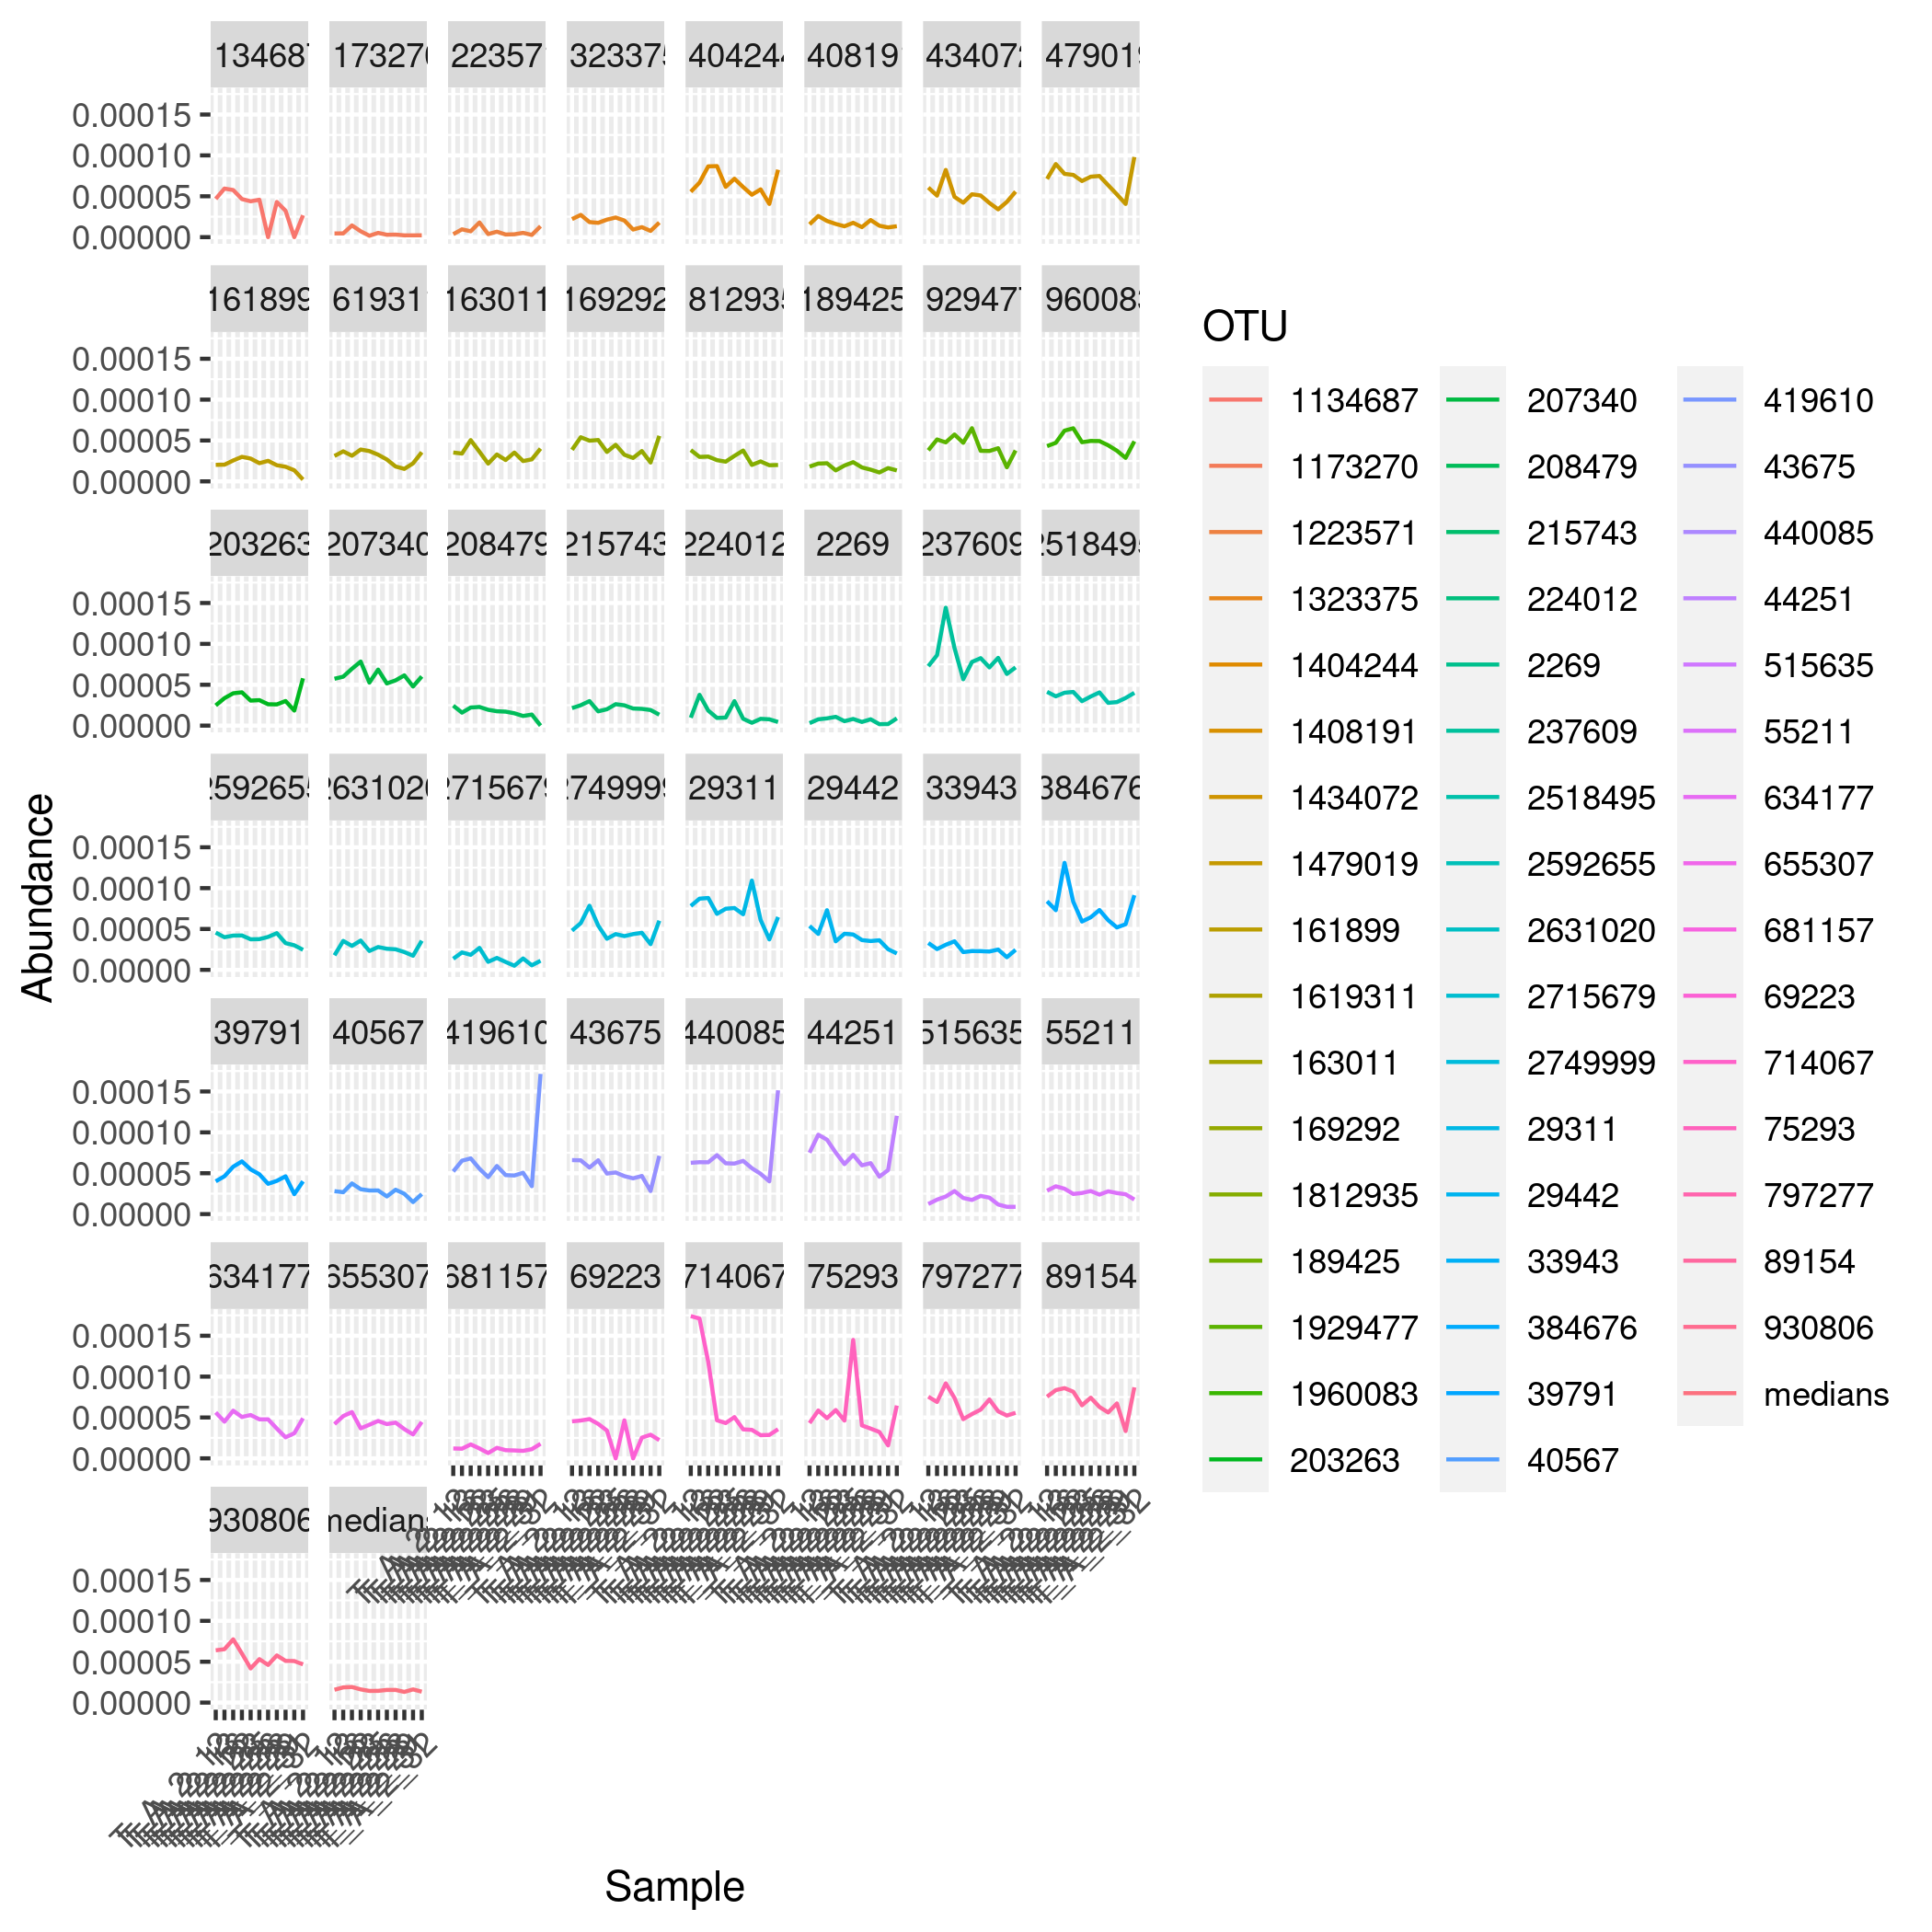
\includegraphics[scale = 0.8]{abundance_tomate_aleatorio1_2.csv_key_otus_medians.png}
   \caption{Plots representing relative abundance of each keystone OTU and one representing the median relative abundance  across samples of rhizosphere of tomate_aleatorio1_2.csv. Most keystone OTUs have relative abundance bigger than the median across all samples.  }
   \label{key_otus_vs_medians_tomate_aleatorio1_2.csv}
\end{figure}
\begin{figure}
 \centering
 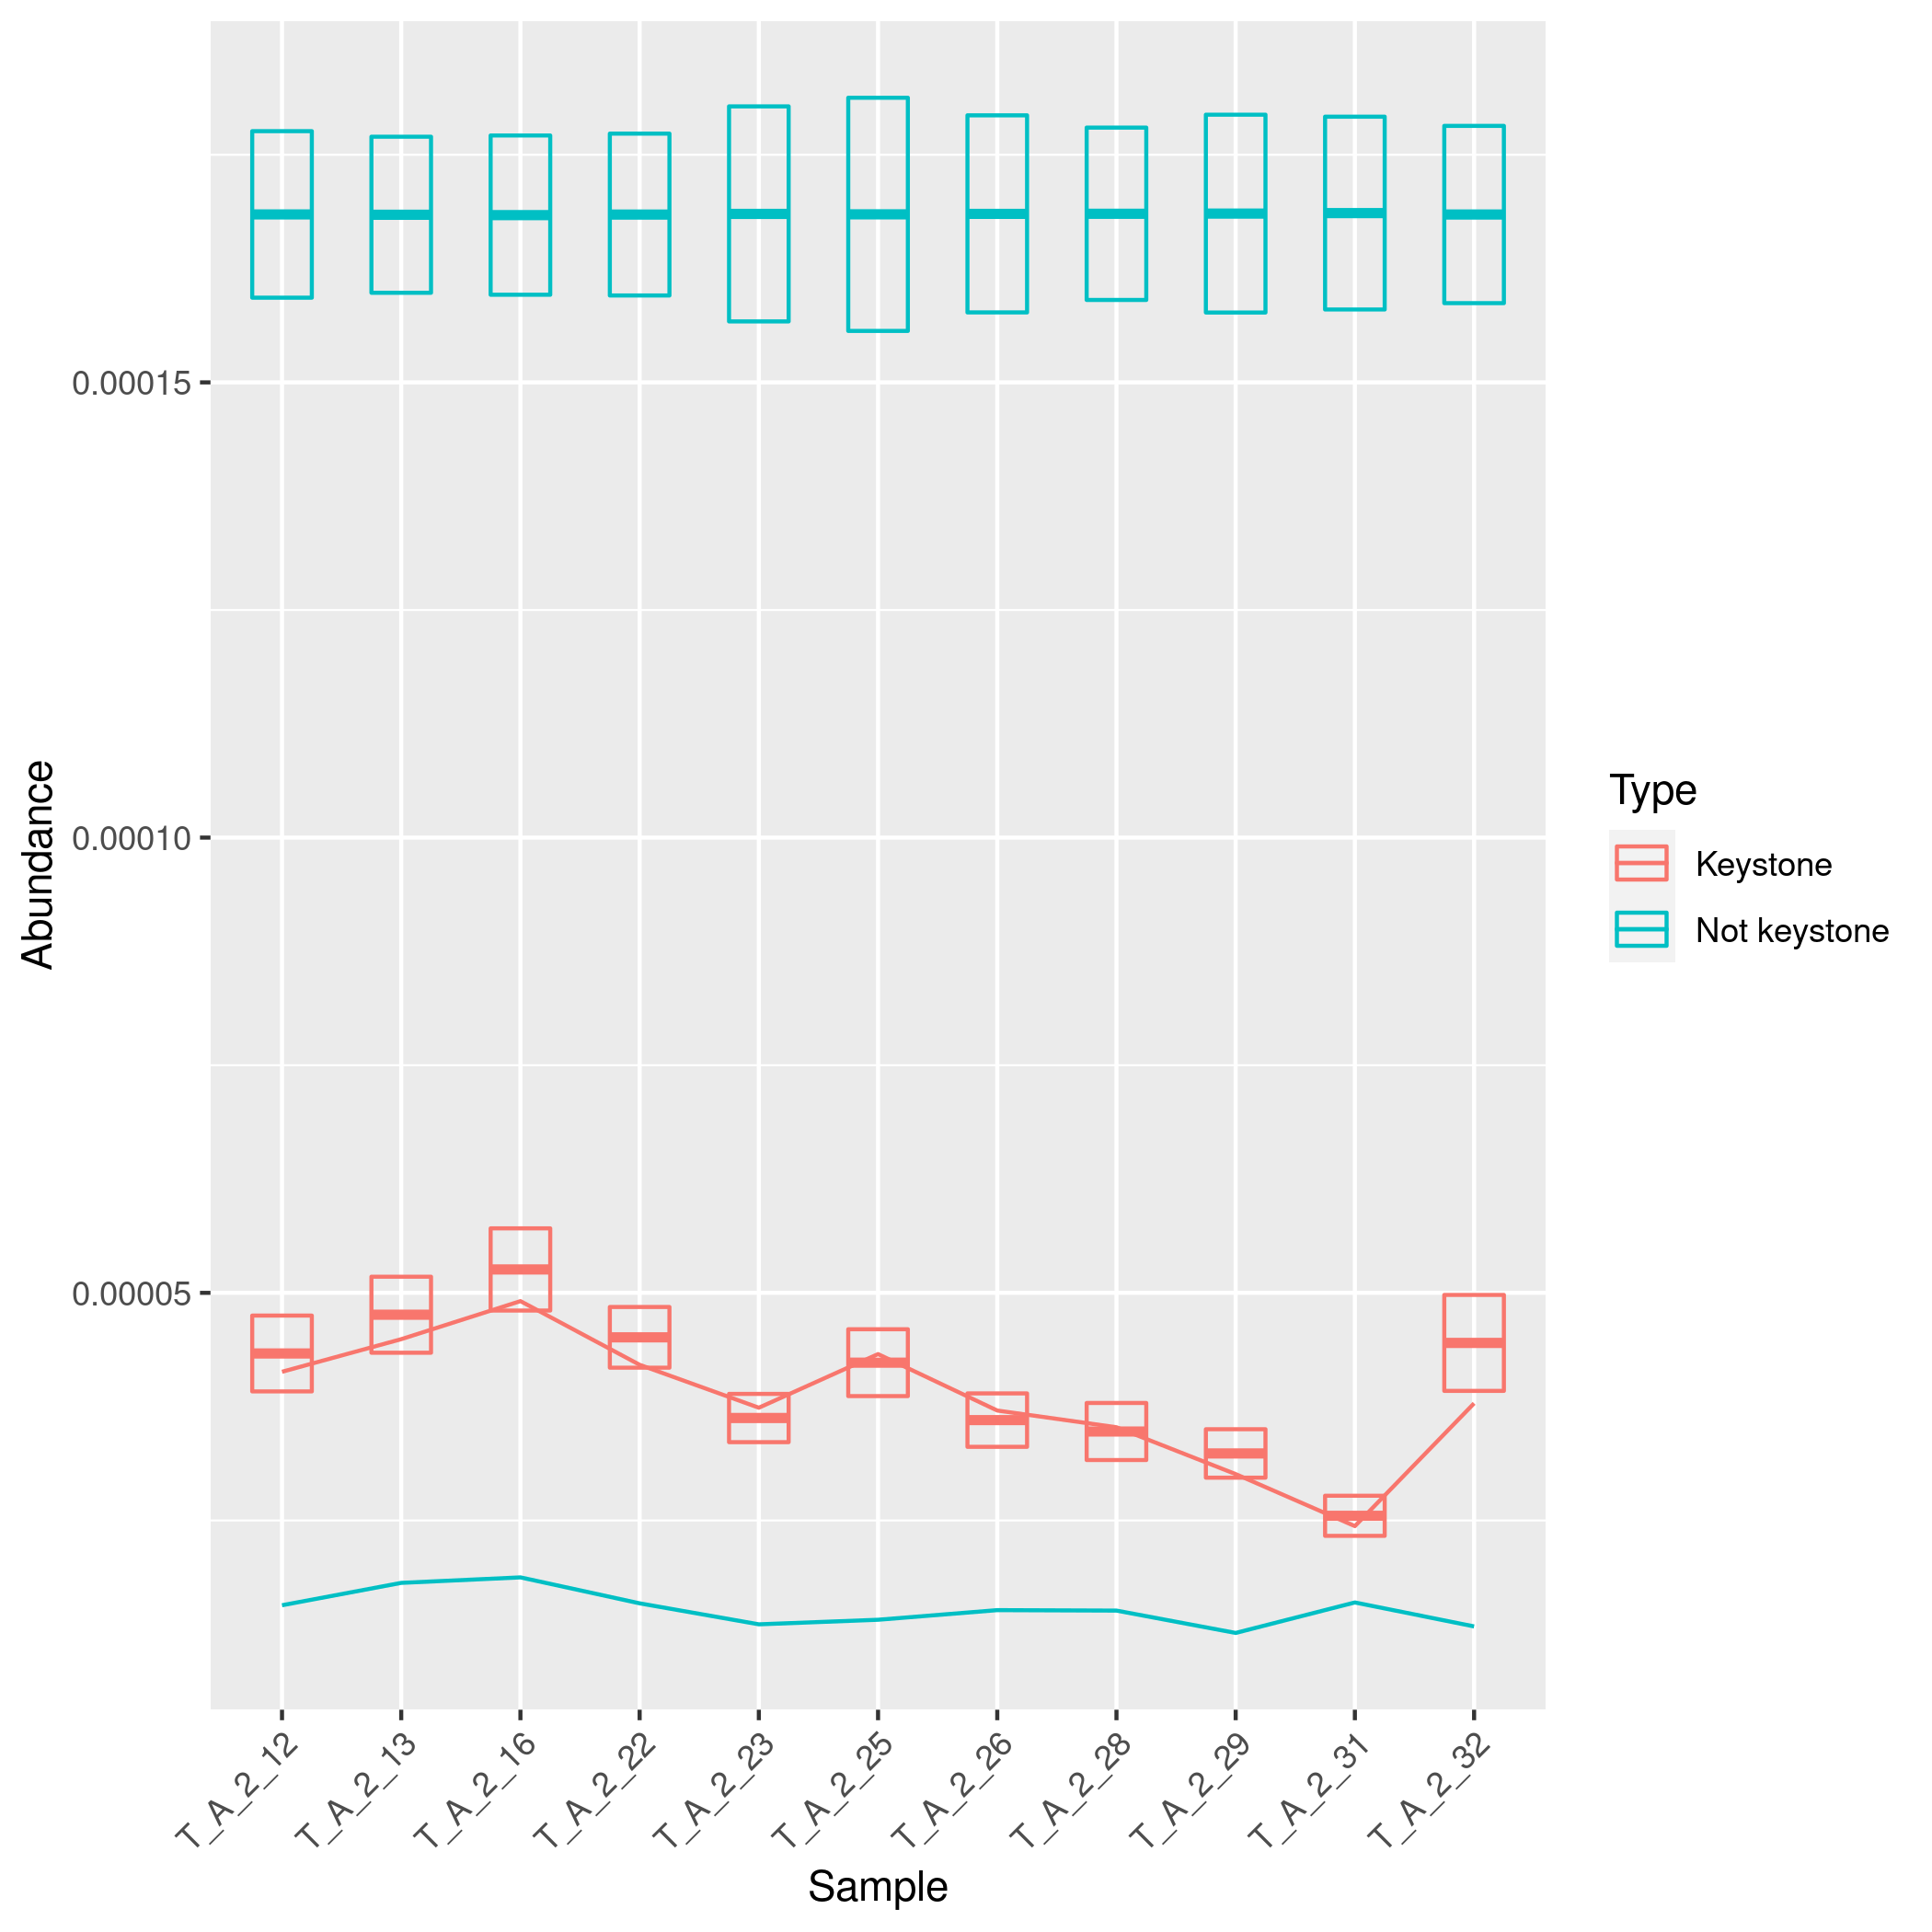
\includegraphics[scale = 0.75]{mean_median_key_vs_not_key_tomate_aleatorio1_2.csv.png}
\caption{Boxes represent mean and standard error in the distribution of corresponding samples. Lines represent the corresponding medians. In these samples of rhizosphere oftomate_aleatorio1_2.csv}
\label{mean_median_tomate_aleatorio1_2.csv}
\end{figure}
\begin{figure}
   \centering
   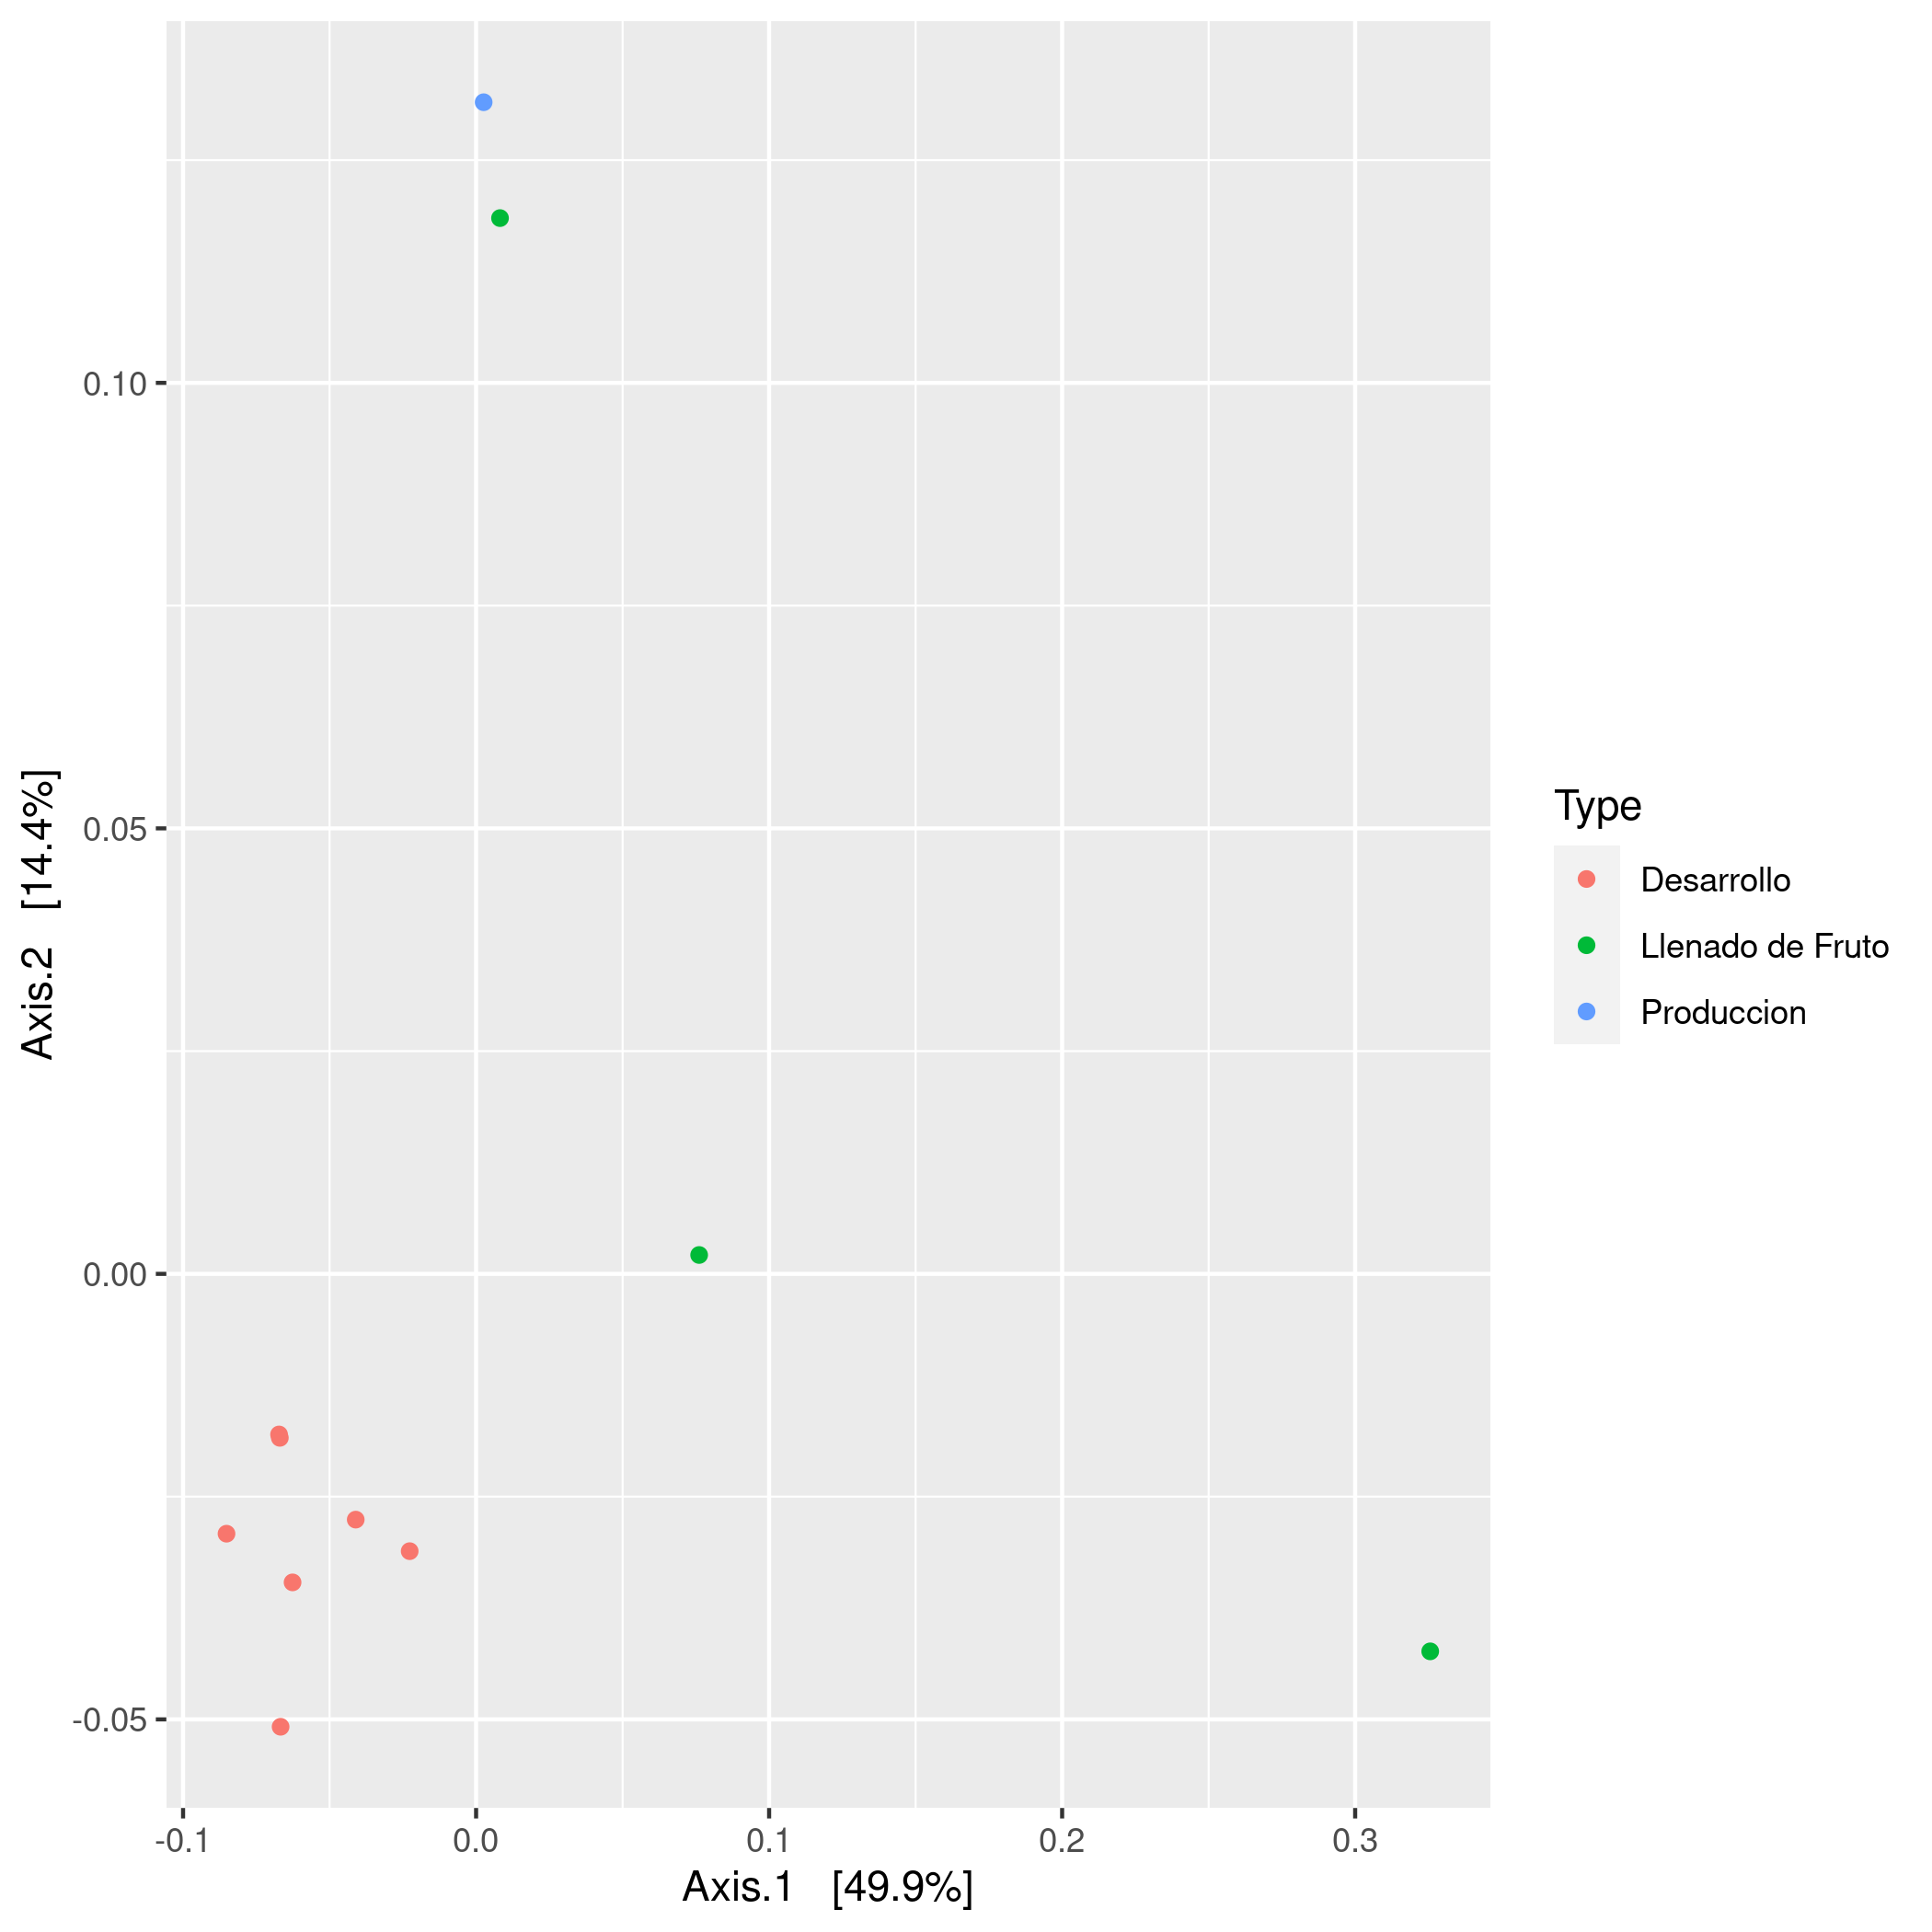
\includegraphics[scale = 0.7]{pcoa_muestras_tomate_aleatorio1_2.csv.png}
 \caption{PCoA analysis with Bray-Curtis distance of rhizosphere samples of tomate_aleatorio1_2.csv.}
 \label{fig:tomate_aleatorio1_2.csv_pcoa}
\end{figure}
\begin{figure}
  \centering
  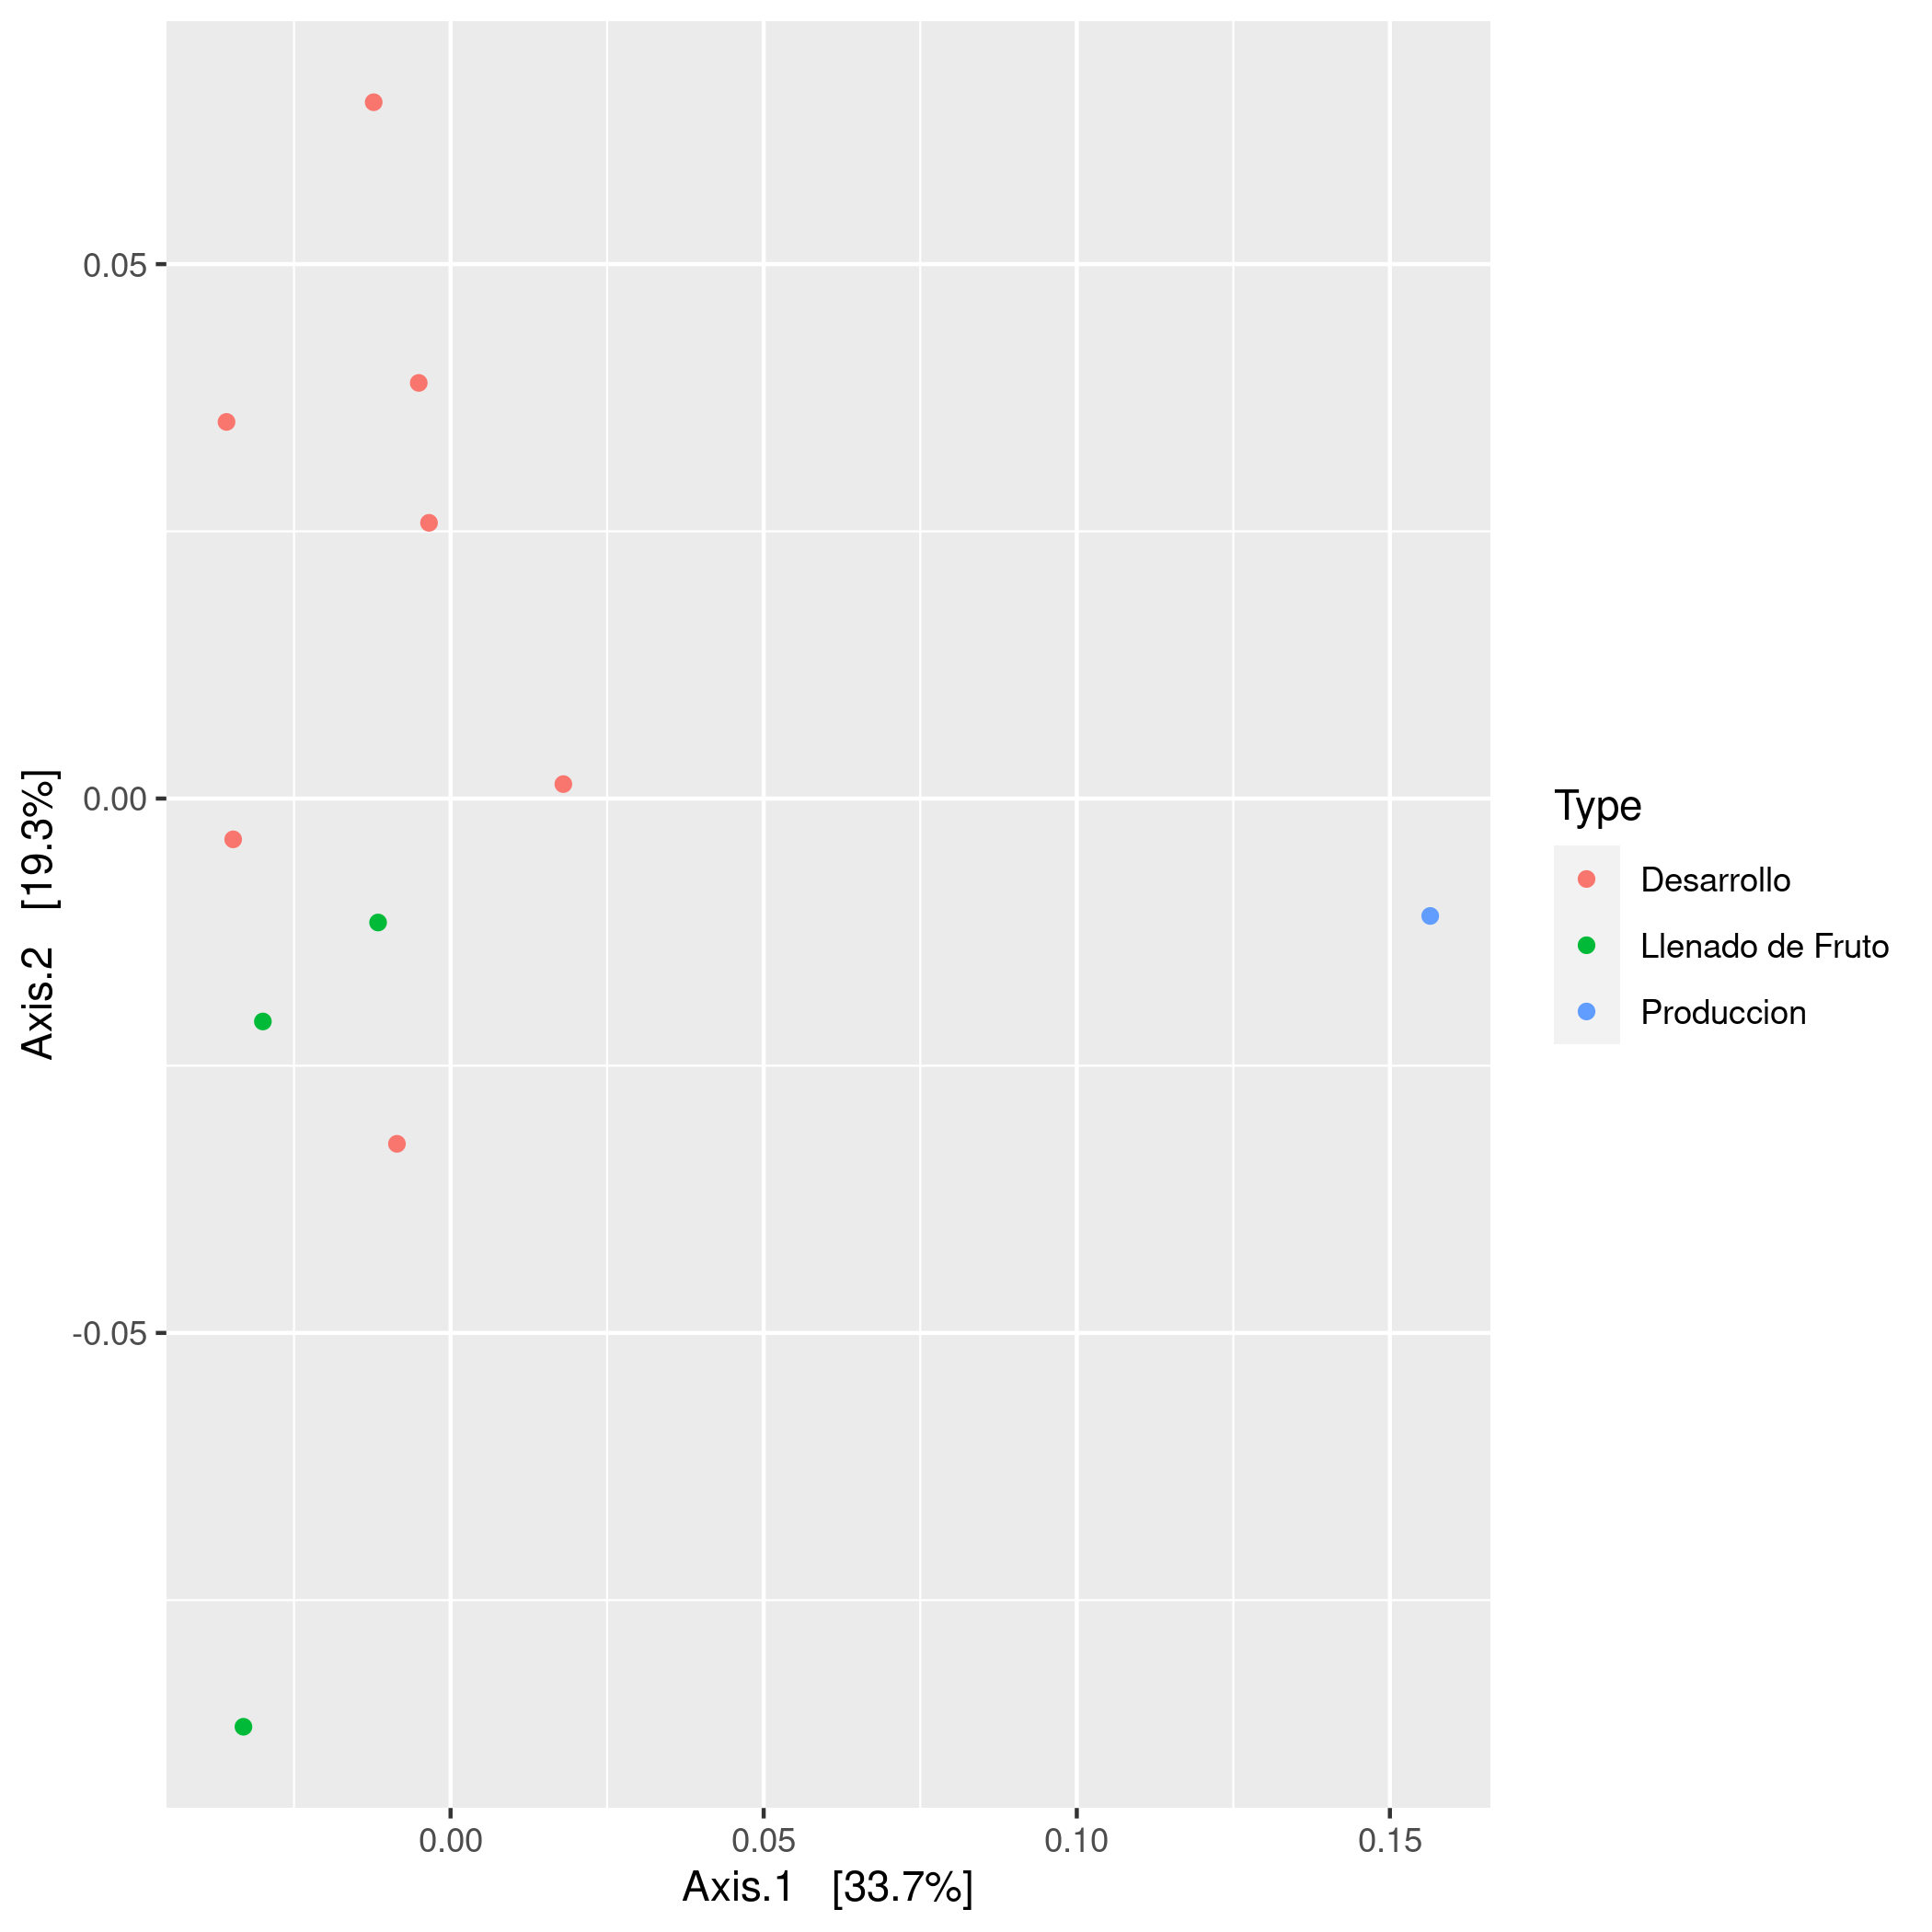
\includegraphics[scale = 0.7]{pcoa_key_otus_tomate_aleatorio1_2.csv.png}
  \caption{PCoA analysis with Bray-Curtis distance of rhizosphere samples of tomate_aleatorio1_2.csv, restricted to keystone OTUs.}
  \label{fig:tomate_aleatorio1_2.csv_pcoa_key_otus}
\end{figure}
